\chapter{Methodik}
\label{chap:method}
Neben der Evaluation von Serverless-Technologie erfüllt Lightbulb Learning auch die Funktion, Erfahrungen mit den methodischen Prinzipien moderner Unternehmensgründung durch deren Anwendung zu sammeln und diese zu bewerten. Dafür werden die Prinzipien einiger Modelle aus diesem Kontext kurz zusammengefasst und deren Umsetzung im Kontext von Lightbulb Learning beschrieben.

\section{Lean Startup}
\label{sec:lean}
\subsection{Die Bauen-Messen-Lernen Schleife}
The Lean Startup ist ein Buch von Eric Ries aus dem Jahre 2011 \cite[vgl.][]{ries2011lean}, welches die Prinzipien der Lean Manufacturing aus der Toyota Kata \cite[vgl.][]{rother2009toyota}, in Kombination mit einigen Prinzipien wie der agilen Entwicklung und dem Design Thinking kombiniert und in den Kontext der schlanken Unternehmensgründung überführt. Im Vordergrund steht der Ansatz, aus Unternehmenssicht validiertes Lernen in den Mittelpunkt zu stellen. Dabei liegt ein besonderes Augenmerk auf dem Weglassen von allem, was nicht für die Validierung benötigt wird, um schnelleres, realistischeres Feedback anstelle von Annahmen als Grundlage für Entscheidungen zurate ziehen zu können. Durch kontinuierliche Weiterentwicklung der Ideen, Experimenten mit realen Kunden und den daraus ableitbaren Schlussfolgerungen soll wiederum das Produkt korrigiert und weiterzuentwickelt werden. Im Mittelpunkt von Lean Startup steht der Ansatz, welcher als Bauen-Messen-Lernen Zyklus \cite[S. 81]{ries2011lean} bezeichnet wird.

\begin{figure}[H]
    \centering
    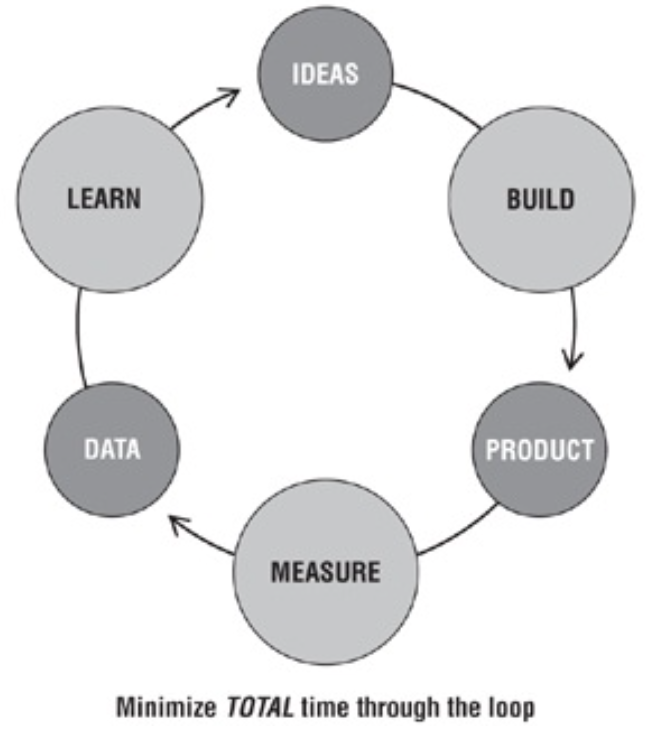
\includegraphics[width = .5\textwidth]{images/lean.png}
    \caption{Build - Measure - Learn Loop, \cite[S. 81]{ries2011lean}.}
    \label{fig:bml}
\end{figure}

\noindent In Abbildung \ref{fig:bml} ist dieser Zyklus visuell dargestellt. Die größeren, helleren Kreise beschreiben dabei Aktivitäten, während die kleineren, dunkleren Kreise Artefakte symbolisieren. Der Beginn des Zyklus ist eine vermutete Hypothese oder Idee zu finden, welche als Ausgangspunkt für die weitere Validierung dient. Diese Idee wird im Bauen-Schritt (build) umgesetzt, dabei ist der Fokus auf der Identifikation des größten Risikos, der Planung eines Tests und der Umsetzung einer Variante der Lösung, die lediglich gut genug ist, um die Idee zu validieren. Im Messen-Schritt wird so objektiv wie möglich untersucht, ob die initiale Hypothese standhalten konnte, und überführt Beobachtungen, Messungen und Ergebnisse in auswertbare Daten. Diese werden dann im letzten Schritt genau analysiert, um eine Einschätzung der Hypothese vorzunehmen, und diese als Grundlage für eine weitere Iteration mit angepasster Hypothese verwendet. Durch dieses Vorgehen können mutige und innovative Technologie- oder Geschäftsentscheidungen getroffen und dabei gleichzeitig das Risiko für Fehlentscheidungen reduziert werden.

\subsection{Minimal funktionsfähiges Produkt (MVP)}
\label{sub:mvp}
Ein Medium für die Umsetzung des Ansatzes ist das minimal funktionsfähige Produkt \cite[vgl.][S. 96]{ries2011lean}, wobei typischerweise die englische Bezeichnung Minimum Viable Product bzw. dessen Akronym MVP verwendet wird. Die Bedeutung des MVP ist, dass eine Produktidee so lange auf den wesentlichen Kern reduziert wird, bis der Umfang so klein ist, das mit wenig Aufwand und somit geringem Risiko validiert werden kann, ob eine Idee funktioniert oder nicht. Scheitert eine Idee so besteht der Erfolg darin, dies früh erkannt zu haben, und somit weitere Ressourcen wie Zeit und Geld nicht wegen dem fehlenden Wissen um den Umstand des Scheiterns vergeudet zu haben. Funktioniert hingegen eine Idee, so kann auch dies früh festgestellt und entsprechend investiert und weiterentwickelt werden. Lightbulb Learning soll wie in dem Buch von Eric Ries beschrieben als MVP entwickelt und früh veröffentlicht werden. Somit soll früh gelernt werden, ob die Idee funktioniert. Tut sie das nicht, so können Änderungen und Experimente durchgeführt werden, welche ihrerseits evaluiert werden und zu weiteren Schlussfolgerungen führen können.

\section{The Mom Test}
\label{sec:mom}
Die von Robert Fitzpatrick in The Mom Test \cite[vgl.][]{fitzpatrick2013mom} beschriebene Methode beschäftigt sich mit der Frage, wie Nutzerinterviews vor der Entwicklung einer Geschäftsidee so strukturiert werden können, dass deren Resultate eine möglichst hohe Objektivität aufweisen. Dabei wird ein besonderer Fokus darauf gelegt, dass die Aussagen von Gesprächspartnern häufig dahingehend verzerrt werden, dass der Interviewer in seinen Annahmen möglichst bestätigt wird. Die Begründung dafür ist, dass vor allem nahestehende Leute, teilweise unterbewusst, lieber etwas Nettes sagen als die Wahrheit. Es werden Techniken beschrieben, die diesen Interpretationsspielraum verringern, um ein genaueres Bild vor der Entscheidung für eine größere Investition von Zeit oder Geld zu erhalten. Die drei hervorgehobenen Prinzipien des Buches lauten:

\begin{enumerate}
    \item „Rede über ihr Leben, und nicht über deine Idee.
    \item Frage nach konkreten Dingen der Vergangenheit, und nicht nach generischen Dingen oder Meinungen über die Zukunft.
    \item Rede weniger, und höre mehr zu.” \cite[S. 128]{fitzpatrick2013mom}
\end{enumerate}

\noindent Um diese Prinzipien anzuwenden, wird beispielsweise vorgeschlagen, in einem Nutzerinterview vorerst gar nicht zu erwähnen, was die eigene Idee ist. Selbst die Information, dass es sich gerade um ein Nutzerinterview handelt, könnte erst im späteren Verlauf andeuten werden, um detaillierte Einblicke in das Leben des Gesprächspartners zu erhalten. Um das zweite Prinzip anzuwenden, könnte beispielsweise nach aktuellen Lösungsstrategien für Probleme gefragt werden, da die subjektive Einschätzung der Größe eines Problems eine Aussage über die Bereitschaft der Nutzung beinhaltet. Sagt ein Gesprächspartner beispielsweise, dass es für ihn ein riesiges Problem ist, und er bereits nach Lösungen dafür gesucht hat, aber noch nicht fündig geworden ist, so kann dies als Bestätigung für die Wahl des richtigen Problems gedeutet werden. Um sicher zu gehen, dass die Problematik wirklich groß genug ist, sollte nach dem zweiten Prinzip nach einer konkreten Investition gefragt werden. Diese muss nicht finanzieller Natur sein, sondern kann auch aus Zeit oder sozialem Aufwand bestehen. Ist ein Gesprächspartner nicht bereit, diese Hürden auf sich zu nehmen, so ist dies wiederum ein starker Hinweis dafür, dass das Problem tatsächlich nicht besonders groß für ihn ist. Mit dem dritten Prinzip wird der Hang adressiert, in eine Diskussion zu verfallen, sich zu rechtfertigen oder sehr stark in den Verkaufsmodus überzugehen. Hier wird unter anderem dazu geraten, am Ende eines Nutzerinterviews, in dem es um die Lebenswelt des Gesprächspartners geht, eine klare Trennung zu machen, und fragend zu formulieren, ob er sich für die eigene Idee interessiert. Dadurch können Anknüpfungspunkte für den späteren Vertrieb des Produkts entstehen, ohne dabei das Verlassen der Objektivität im vorhergehenden Gesprächsabschnitt zu riskieren.

\section{Anforderungen an die Werkzeuge}
\label{sec:reqtools}
In diesem Abschnitt geht es um die Anforderungen, welche die ausgewählten Werkzeuge wie Technologien und Methoden erfüllen müssen, um für die Entwicklung von Lightbulb Learning infrage zu kommen. Die Rahmenbedingungen dafür sind die Entwicklung eines vollständigen digitalen Produkts, von der Entwicklung der Idee, über die Ausarbeitung des Produktdesigns bis hin zur Umsetzung, Qualitätssicherung und dem Betrieb der Software. In den Bereich der Qualitätssicherung fällt sowohl das Schreiben von automatisierten Tests, welche einen definierten Funktionsumfang abdecken, aber auch die Validierung der Idee selbst, der Usability, der Datensicherheit und des Geschäftsmodells. Entsprechend dem breiten Spektrum der Problemfelder wird ein breites Spektrum an Werkzeugen genutzt. Auch der Umstand, dass sich der personelle Rahmen auf eine Person beschränkt, und somit die Verteilung der Kompetenzten auf die Breite und folglich nicht auf die Tiefe bedingt, konkretisiert die Anforderungen an die verwendeten Werkzeuge. Eine weitere Dimension für die Anforderungsanalyse ist die zeitliche: Innerhalb einiger Monate wird ein lauffähiges, validiertes und sinnvolles minimal-funktionsfähiges Produkt entwickelt, was eigene Limitationen mit sich bringt. Es lässt sich zusammenfassen: Alle verwendeten Werkzeuge müssen mit einer steilen Lernkurve einher gehen, eine hohe Kompatibilität zueinander aufweisen und in ihrer Summe das gesamte Spektrum von technologischen, methodischen, gestalterischen oder wirtschaftlichen Problemfeldern abdecken.

\subsection{Prinzip der Einfachheit}
Die verwendeten Werkzeuge fußen allesamt auf den agilen Prinzipien \cite[vgl.][]{beck2001}, allen voran dem zehnten agilen Prinzip: „Einfachheit -- die Kunst, die Menge nicht getaner Arbeit zu maximieren -- ist essenziell” \cite[10. Prinzip]{beck2001}. Unter der Zuhilfenahme möglichst guter Werkzeuge für die Aufwandsminimierung sollen die Anforderungen zufriedenstellend erfüllt werden.

\subsection{Lightbulb Learning als MVP}
Der Fokus auf den Aufgabentypen \emph{offene Frage} ist im Lichte des Prinzips der Einfachheit zu sehen: Es ermöglicht eine Validierung des Produkts, erfordert aber nicht die Umsetzung größerer Komplexität wie es beispielsweise automatisiert bewertbare Programmieraufgaben oder Dateiuploads tun würden. Ab einem möglichst frühen Zeitpunkt soll eine funktionierende Version des Produkts online zur Verfügung zu stehen, welches von Nutzern ausprobiert werden kann. Dieser Fokus ist ein Resultat aus dem ersten der zwölf agilen Prinzipien: „Unsere höchste Priorität ist es, den Kunden durch frühe und kontinuierliche Auslieferung wertvoller Software zufrieden zu stellen“ \cite[1. Prinzip]{beck2001}. Der Fokus auf funktionierende Software als das wichtigste Fortschrittsmaß führt zu einer realistischen Einschätzung des aktuellen Stands und der verbleibenden Ziele im Sinne des Fortschritts der Thesis und des Produkts Lightbulb Learning, und der Korrektheit der Richtung. Technologisch wird Serverless-Technologie eingesetzt, da diese durch technische Abstraktion die Schwelle hin zu funktionierender und bereitgestellter Software senkt. So sollen mit Serverless-Technologien beispielsweise die Themen der Benutzerverwaltung, der Datenpersistenz, der Sicherheit und Zugreifbarkeit auf diese Daten sowie der Aufbau einer Continuous Deployment Pipeline, das Hosting einer Web-Applikation und die Skalierung all dieser Aspekte abgebildet werden. Somit kann die Idee validiert werden, ohne langwierige Entwicklung oder hohe Entwicklungskosten durch größere Teams in Kauf nehmen zu müssen. Eine detaillierte Beschreibung evaluierter und verwendeter Serverless-Komponenten befindet sich in Kapitel \ref{chap:serverless}.

\subsection{NoCSS Framework}
Eine weitere Anforderung an die Entwicklung von Lightbulb Learning ist die Entwicklung einer Designsprache, woraus die Anforderung an das Werkzeug resultiert, diese möglichst einfach, konsistenz und allgemeingültig zu erstellen und weiterzuentwickeln. Die Form dieser Designsprache soll dabei explizit über Vektorgrafiken in Designwerkzeugen wie Figma oder Sketch hinausgehen, und stattdessen einsatzfähiger HTML und CSS Code sein. Die Klasse an Frameworks, welche diese Anforderungen erfüllt, werden NoCSS-Frameworks genannt.
